
%
%	Preamble of Master Thesis 
%	TODO adaption to cismet layout
%
%	KOMA-Script Dokumentklasse "scrbook"

% prints warnings about obsolete syntax and syntax which will probably break
\RequirePackage[l2tabu, orthodox]{nag}

\documentclass[12pt, pdftex, a4paper, bibliography=totoc, listof=totoc, parskip=half]{scrreprt}

% use T1 Fonts
% The Latin Modern fonts are enhanced versions of the Computer Modern fonts. They have enhanced metrics and glyph coverage.
\usepackage{lmodern}
\usepackage[T1]{fontenc}

% use utf8 as encoding
\usepackage[utf8]{inputenc}

% Language configuration
% quotes
\usepackage{csquotes}

% comment out, which is not needed
\usepackage[english]{babel}
%\usepackage[ngerman]{babel}

% mathematical symbols
\usepackage{amssymb}

%%%% === Verzeichnisse (TOC, LOF, LOT, BIB) ===
   %liststotoc,      % Tabellen & Abbildungsverzeichnis ins TOC
   %idxtotoc,        % Index ins TOC
   %bibtotoc,         % Bibliographie ins TOC
   %bibtotocnumbered, % Bibliographie im TOC nummeriert
   %liststotocnumbered, % Alle Verzeichnisse im TOC nummeriert 

\usepackage{color} 
\definecolor{lightgray}{rgb}{.9,.9,.9}
\definecolor{darkgray}{rgb}{.4,.4,.4}
\definecolor{purple}{rgb}{0.65, 0.12, 0.82}


% use longtables
\usepackage{longtable}

% tables
% booktabs - The pack­age en­hances the qual­ity of ta­bles in LaTeX, pro­vid­ing ex­tra com­mands as well as be­hind-the-scenes op­ti­mi­sa­tion. 
\usepackage{booktabs}

% graphics in tables
% \usepackage{picins}
% \usepackage{array}

%Einbinden von Grafiken in Tabellen HIER
%\usepackage{here}


% format for tables and image descriptions
\addtokomafont{caption}{\small\bfseries}
\addtokomafont{captionlabel}{\bfseries}
 
% line spacing 1,5
\usepackage{setspace}
\onehalfspacing

% page settings
\usepackage{geometry}
\geometry{a4paper,left=35mm,right=25mm,%
bottom=25mm,top=25mm,bindingoffset=5mm,%
includehead,includefoot
}
% allow landscape pages
\usepackage{pdflscape}

%Fußnoten durchlaufend nummerieren
\usepackage{chngcntr}
\counterwithout{footnote}{chapter}

\pagestyle{headings}
% Eigene Kopfzeile
%\usepackage{scrpage2}
%\pagestyle{scrheadings}
%\automark[section]{chapter}


% url – Ver­ba­tim with URL-sen­si­tive line breaks
\usepackage{url}

%PDF Version 1.6
\pdfminorversion=6

% for inserting graphics
\usepackage{graphicx}

% for inserting graphics as background picture
\usepackage{eso-pic}

\usepackage{tocbasic}

% configuration bibliography

% As backend use biber
% Biber: A BibTeX replacement for users of BibLaTeX
% Deals with the full range of UTF-8 
% http://biblatex-biber.sourceforge.net/
	
%\usepackage[backend=biber,style=numeric]{biblatex} %[5]
\usepackage[backend=biber,style=alphabetic]{biblatex} %[JW86]

% more styles can be found in the deocumentation of biblatex

\bibliography{bibArchive/libarchive}


\usepackage{color}
\usepackage{xcolor}
\usepackage{listings}
\usepackage{caption}

\DeclareCaptionFont{white}{\color{white}}
\DeclareCaptionFormat{listing}{\colorbox{gray}{\parbox{\textwidth}{#1#2#3}}}
\captionsetup[lstlisting]{format=listing,labelfont=white,textfont=white}

%----------------------------------
%----------JavaScript--------------
%----------------------------------
\lstdefinelanguage{JavaScript}{
  keywords={typeof, new, true, false, catch, function, return, null, catch, switch, var, if, in, while, do, else, case, break},
  keywordstyle=\color{blue}\bfseries,
  ndkeywords={class, export, boolean, throw, implements, import, this},
  ndkeywordstyle=\color{darkgray}\bfseries,
  identifierstyle=\color{black},
  sensitive=false,
  comment=[l]{//},
  morecomment=[s]{/*}{*/},
  commentstyle=\color{purple}\ttfamily,
  stringstyle=\color{blue}\ttfamily,
  morestring=[b]',
  morestring=[b]"
}

\lstset{
	    language=JavaScript,
         basicstyle=\footnotesize\ttfamily, % Standardschrift
         numbers=left,               % Ort der Zeilennummern
         numberstyle=\tiny,          % Stil der Zeilennummern
         %stepnumber=2,               % Abstand zwischen den Zeilennummern
         numbersep=5pt,              % Abstand der Nummern zum Text
         tabsize=2,                  % Groesse von Tabs
         extendedchars=true,         %
         breaklines=true,            % Zeilen werden Umgebrochen
         keywordstyle=\color{red},
    		frame=b,         
 %        keywordstyle=[1]\textbf,    % Stil der Keywords
 %        keywordstyle=[2]\textbf,    %
 %        keywordstyle=[3]\textbf,    %
 %        keywordstyle=[4]\textbf,   \sqrt{\sqrt{}} %
         %stringstyle=\color{blue}\ttfamily, % Farbe der String
         showspaces=false,           % Leerzeichen anzeigen ?
         showtabs=false,             % Tabs anzeigen ?
         xleftmargin=17pt,
         framexleftmargin=17pt,
         framexrightmargin=5pt,
         framexbottommargin=4pt,
         %backgroundcolor=\color{lightgray},
         showstringspaces=false      % Leerzeichen in Strings anzeigen ?        
 }

\def\inline{\lstinline[basicstyle=\ttfamily,breaklines=true,breakatwhitespace,keywordstyle={}, 
literate=  {\\\-}{}{0\discretionary{}{}{}}]}


%-----------Abkürzungsverzeichnis---------------

\usepackage[intoc]{nomencl}
% Befehl umbenennen in abk
%\let\abk\nomenclature
% Deutsche Überschrift
%\renewcommand{\nomname}{Abkürzungsverzeichnis}
% Punkte zw. Abkürzung und Erklärung
\setlength{\nomlabelwidth}{.20\hsize}
\renewcommand{\nomlabel}[1]{#1 \dotfill}
% Zeilenabstände verkleinern
\setlength{\nomitemsep}{-\parsep}
\makenomenclature

%-----------------------------------------------

%----------------------------------
%----------Neue Kommandos----------
%----------------------------------

\newcommand{\myfig}[1]{Abbildung~\vref{#1}}
\newcommand{\mytab}[1]{Tabelle~\vref{#1}}
\newcommand\todo[1]{\textcolor{red}{TODO: #1}}
\hyphenation{TODO}

%add the end of the line '\tabularnewline' has to be used insted of '\\'
\newcommand{\head}[1]{\centering \textcolor{white}{\textbf{#1} }}
\newcommand{\tableSection}[1]{\multicolumn{3}{|l|}{\rowcolor[gray]{0.9}\textbf{#1}}}

%Percent Value
\newcommand{\per}[1]{{#1}\,\%}


% hyperref should be one of the last imported packages
% although there are exceptions: http://tex.stackexchange.com/questions/1863/which-packages-should-be-loaded-after-hyperref-instead-of-before
% varioref – Intelligent page references
\usepackage{varioref}

\usepackage{hyperref}

% remove ugly red boxes around the hyperrefs
\hypersetup{%
    pdfborder = {0 0 0}
}


%----------------------------------
%----------------------------------
%----------------------------------


%
%	EOF
%

\title{%
\large Master Thesis\\
\\[20mm]
{\LARGE Integration of Web UI Technologies in cids Navigator}\\[30mm]
}


\author{%
Daniel Meiers\\
Matriculation.No.: 3538990\\
daniel.meiers@cismet.de\\[15mm]
First Examiner: Denzer /Guettler\\
Second Examiner: Guettler / Denzer\\
Adivisors: Thorsten Hell\\[20mm]
}

\newcommand{\HRule}{\rule{\linewidth}{0.5mm}}

\begin{document}

%\maketitle

\begin{titlepage}
\begin{center}

% Upper part of the page. The '~' is needed because \\
% only works if a paragraph has started.

\includegraphics[width=0.5\textwidth]{img/logo}~\\[1cm]

\textsc{\LARGE Master Thesis}\\[1.5cm]

% Title
\HRule \\[0.4cm]
{ \huge \bfseries Master Thesis Thema \\[0.4cm] }

\HRule \\[1.5cm]

\textsc{\Large Daniel Meiers}\\[0.2cm]
\textsc{\Large Matriculation No.: 3538990}\\[0.2cm]
\textsc{\Large daniel.meiers@cismet.de}\\[4cm]

% Author and supervisor
\begin{tabular}[0.8\textwidth]{l l}
\emph{First Examiner:} & Prof. Dr. Ralf \textsc{Denzer} \\
\emph{Second Examiner:} & Prof. Dr. Reiner \textsc{Güttler} \\
\emph{Advisors:} & Martin \textsc{Scholl}, Dipl. Inf. (FH) \\
 				& Sascha \textsc{Schlobinski}, M.Sc.
\end{tabular}


\vfill

% Bottom of the page
{\large \today}

\end{center}
\end{titlepage}  
 
 
 
\tableofcontents


% insert provisional TOC here TODO: remove this and insert it in the respective chaptersls

%\chapter{Abstract}
%\chapter{Introduction}
%	\section{Problem Description}
%	\section{Objectives}
%	\section{Conventions}

%\chapter{Conception}
%	\section{Java Web Components}
%		\subsection{requirements}
%		\subsection{apis}
%		\subsection{testing}
%	\section{Web Framework examination}
%		\subsection{Web Development - State of the Art}
%			\subsubsection{Web 2.0, HTML5, AJAX}				
%			\subsubsection{MVC}
%			\subsection{templates}
%			\subsection{dependendy management}	
%			\subsection{testing / debugging}
%		\subsection{Requirements} 
%		what do we exactly excpect/need from the frameworks? 
		\chapter{Comparison of modern Java Script Frameworks}

%\section{Open Questions}

%just for me....
%\begin{itemize}
%	\item Security issues of templating systems (especially XSS)
%	\item differences of dom based vs string based templates
%	\item is there a difference between templates and data binding?
%\end{itemize}
 
\section{Overview}

\autocite{Doe:2009:Online} There is a huge and steadily increasing amount of new JS MV* (the * stand for C=Controller, VM=ViewModel, W=Whatever fits best to you) frameworks. 
%(prove this with literature, show both pictures of ToDoMVC App). 
A good overview over existing projects is provided by the Todo MVC App [Quelle TodoMVC]
The Todo MVC app was created with the intention to help developers selecting a JavaScript framework, by providing implementations of the very simple and ever same 
ToDo App, which allows to define a set of tasks that need to be done. 
%The application allows to add/delete/edit todo tasks and to mark/unmark tasks as done/undone. 
The TodoMVC app gives also a good evidence of the rapid increase of existing JavaScript MVC frameworks. Figure \ref{fig:todoMvcComp} shows a screenshot of the ToDoMVC taken at two different dates with a period of a year.

\begin{figure}
	\centering	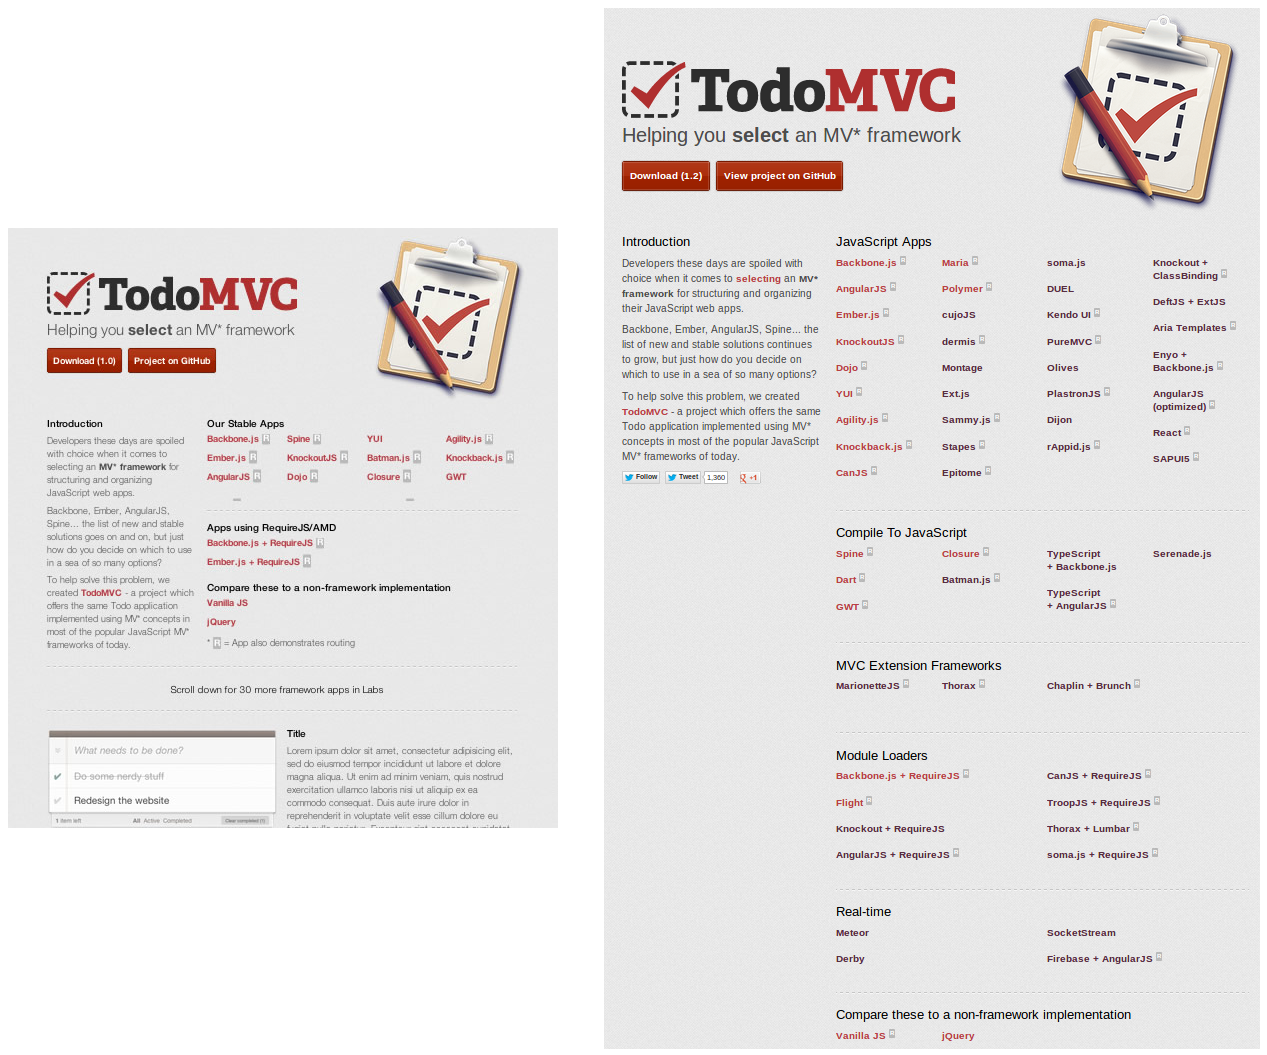
\includegraphics[width=1.0\textwidth]{./img/todo_mvc_app_comparison.png}
	\caption{Screenshot TodoMVC app left:July 2012, right: August 2013~}
	\label{fig:todoMvcComp}
\end{figure}
    

The large amount of different frameworks makes it impossible to examine them all in detail. Therefore a two step approach to filter the best suiting candidate is applied. In a first step a very rough comparison of the frameworks is made to filter out the most inappropriate frameworks. The remaining frameworks are then examinied in more detail in chapter \ref{chap:detail_comparison}. Furthermore a simple application is implemented with the each of the frameworks to get a better understandig and to allow a comparison of them. The implement application is a Simple Greeting Application where a user can edit its First and Last Name and sees a greeting.  

%The implemented application is a simple cids renderer for an example vermessungriss bean taken from wunda. This example was choosen since such renderer are one part that will be implemented in future.    

The following list shows relevant JS MV* frameworks taken from the ToDoMVC app. The list only contains frameworks wich are available in a stable release (at least 1.0.0), availabe as open source. Furthermore a combinations of different apis are also excluded. 

\begin{itemize}
	\item Dojo
	\item YUI
	\item CanJS
	\item soma.js
	\item Maria
	\item Backbone JS
	\item AngularJS
	\item Ember JS
	\item Knockout JS
\end{itemize}

Dojo as well as YUI (Yahoo! User Interface) arent MV* frameworks in the proper meaning of an MV* Framework. They are, like JQuery, DOM/Ajax wrapping libraries. Both has several addiational features like ui-elements, effects and animations. Both doesn't provide components that implement MVC pattern and don't provide the user with built in features like data binding, templating or routing and are therefore not taken into further considerations.


CanJS, Soma.js and Maria are very new MVC Frameworks all providing a different set of features and a different emphasis. 


According to [http://de.slideshare.net/moschel/canjs-the-best-of-both-worlds] CanJS combines the best features of lightweight frameworks like BackboneJS, which are easy to learn and have a small size, as well as of heavy frameworks like EmberJS which offer a lot of good features like live binding,computed properties and memory safety. CanJS can use EJS or Mustache as templating engines which are both string based templating engines. In one sentence CanJS can be characterized through its high performance, its memory leak prevention and the fact that it can be used with a lot of different DOM libraries. 


Although soma.js can be used as a MVC framework, the basic idea behind soma.js is a more general and architectural approach. "soma.js  provides tools to create a loosely-coupled architecture broken down into smaller pieces." [soma website] In order to do so, it implements a large set of different design patterns, like dependency injection, observer pattern or mediator pattern. Soma.js implements its own template engine based on soma.js. The more architectural bias makes it less comfortable for the developer to work with soma.js since a lot of work needs to be done manually that other frameworks do automatically. 


The authors of Maria emphasize that the framework implements the "real" MVC pattern. Maria is a very leightweight framework which means that there is no built in support for templates and data binding. Similarly to soma.js, working with Maria means to write a lot of boilerplate code. 


Generally speaking, the biggest problem with the above mentioned very young frameworks is, that these projects are not so well documented and there is only a small community which makes it very difficult to find information or help when problems occur. This disqualifies these frameworks as possible candidates.


One of the more matured and proven frameworks is Backbone JS. A lot of really large and impressive projects are built with backbone.js such as LinkedIn, AirBnB, Trello or FourSquare. Hence its maturity, it is well documented and there is a large and active community which makes it easy to find help. Backbone JS  consists of different components concerning all necessary aspects of building single page web application such as models, views and routers. Thus application built with backbone normally have a clear defined strucutre [heise developer backbone article]. Backbone has built in support for persisting model data to REST apis. To make this built in component to work properly it is necessary to have a correlation of your model names and the REST api paths. The backend connection can be implemented manually if the standard one is not suited. There are already some exisiting Modules that do this like Backbone.localstorage which stores all data in the Browser itself. 


An adverse is, that Backbone JS is not able to reflect changed model data to the view automatically (and vice versa). Backbone's approach to achieve this is much more leightweight. Each model can fire a set of events. A backbone view can listen to these events. Each view has a render function, which generates the html for displaying the view. This function needs to be implemented manually for each view. This approach allows it to use any templating engine. Since backbone needs the dependency to underscore, you can use the templating function from this library. Another drawback is that backbone does not manage the display of different views. Admittedly it provide you with a router object, but again, this objects just defines what function should be executed when a route is loaded. The developer has to initialze the new view and to destroy all views no longer needed. There is always the danger of memory leaks which causes several performance and security issues. At least, using backbone means a lot of initialisation overhead, since it is first necessary to define the domain model and set up the infrastructure. Considerin all this disqualifies Backbone JS as possible candidate.       


The remaining 3 Frameworks does not have any of the above mentioned drawbacks and are used for a much more detailed examiniation described in the following chapter.

\section{Comparison of AngularJS, EmberJS and KnockoutJS}\label{chap:detail_comparison}

\subsection{Knockout JS}

Knockout JS is a more leightweight library, which emphasis is to implent the MVVM (Model-View-ViewModel) pattern for HTML. This pattern enables HTML with two way data binding and a seperation of gui logic/state from the gui itself.


The two way data binding is implemented by using special Java Script Objects (Knockout Observables) and a special html attribute both provided by Knockout. Thus model changes are automatically reflected to the view. The following example demonstrates how to bind a property of a viewmodel to an html textfield element.


\begin{lstlisting}[label=knockout_js][caption=the ViewModel]
function ViewModel(){
	this.firstName = ko.observable('Daniel');
	this.lastName = ko.observable('Meiers');
	this.fullName = ko.computed(function({
				return this.firstName()+" "+this.lastName();
			},this); 
}
ko.applyBindings(new ViewModel());
\end{lstlisting}

\begin{lstlisting}[caption=the html view]
 	<div>
		<label>First Name</label> 
		<input type="text" data-bind="value: firstName">
	</div>
	<div>
		<label>Last Name</label> 
		<input type="text" data-bind="value: lastName">
	</div>
	<p data-bind="text: 'Hello '+fullname"></p>
\end{lstlisting}

The data-bind attribute of the input element tells Knockout to bind the ViewModels property to an attribute of the containing element (in this case the value attribute of the input element). There is a large set of predefined bindings for different purposes. There are controlling and appearance bindings such as the vissible or the style binding, control flow bindings such as the foreach binding to iterate over a set of ViewModel properties and at least, form fields bindings. If these bindings are not sufficient it is possible to create custom bindings.

%picture inserted here because otherwise it will interrupt the listings above
\begin{figure}[h]
	\centering	
	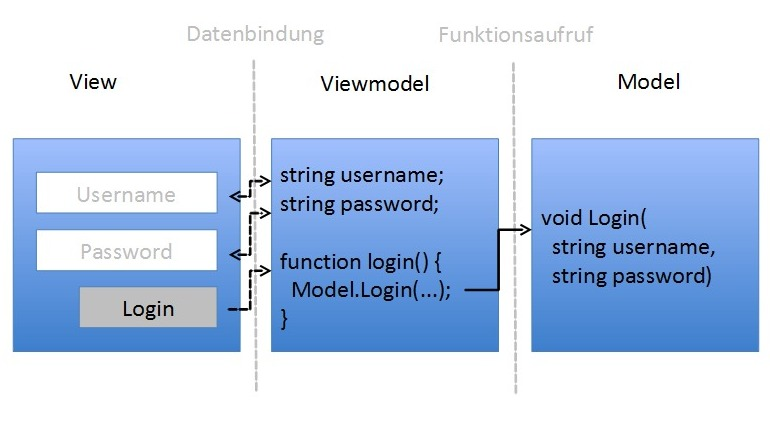
\includegraphics[width=0.7\textwidth]{./img/mvvm.jpeg}
	\caption{MVVM pattern, source heise developer knockout article}
	\label{fig:mvvm}
\end{figure}


The last line in listing XY binds the ViewModel to the view. After that all changes in the ViewModel are reflected to the input element and vice versa. The ViewModel itself defines two different sort of properties. The properties 'firstName' and 'lastName' are normal observables. The 'fullName' property is a computed observable which can be any calculated value, also considering other observables. Since the properties are special Knockout objects, it is necessary to access the property values like a function (see line 5 in listing \ref{knockout_js}).


Knockout also provides a more convienent way to define the properties of a viewModel, the mapping plugin. The mapping plugin converts any property of any JSON object to Knockout observable in order to act as ViewModel. The following listing (\ref{ko_mapping}) shows the above introduced name example with the mapping plugin.

\begin{lstlisting}[label=ko_mapping][caption=the mapping plugin]
var person = {
	firstName : 'Daniel';
	lastName : 'Meiers';
	fullname : function({
			return firstname +lastName;
		});
var viewModel = ko.mapping.fromJS(person);
\end{lstlisting}


Knockout JS doesn't support you by attaching a server side backend. Furthermore it is not able to route between different pages of your application. Thus these parts of the SPA has to be implemented by your own or with additional Frameworks.


\subsection{Ember JS}

Ember JS is one of the younger frameworks out there, mainly created by Yehuda Katz and Tom Dale and introduced in December 2011 (see link yehuda katz blog). In this short time Ember JS could make a really impressive progress and has gained a lot of attraction (github forks, stars, watches). It comprises all necessary parts for building web applications including two way data binding with templates, a routing mechanism and provides a way to connect the application to REST API's. 

Ember is a very stringent and opinionated framework and is built upon concepts such as DRY (dont repeat yourself) and CoC (Convention over Configuration). Especially the usage of naming conventions allows it to write applications with a nominal amount of code. The disadvantage of this is that it is more sophisticated to get started with Ember.js because you have to get into the Ember philosohy. %(TODO rewrite this)
Furthermore this makes Ember one of the largest framewworks (56kb)


It uses Handlebars as its templating engine, which is a very popular string based templating enginge. Ember.js also provides a way to connect your application to RESTful WebServices with an additional project Ember-Data. As well as Ember itself, Ember-Data makes highly use of the Convention over Configuration principle which means that Ember-Data expects the data provided by a REST-Service in a special format. The Ember team substantiate : "[...]we don't think most web developers should have to write any custom XHR code for loading data. Strong conventions on the client and strong conventions on the server should allow them to communicate automatically." (Ember website stabilizing ember data). Besides Ember-Data it is also possible to use any other server connection implementation.         


To build an Ember application it is first necessary to create an instance of an Ember Application (see listing \ref{em_js}).
\begin{lstlisting}[label=em_js, caption=app.js]
var App = Ember.Application.create();
\end{lstlisting}

\begin{lstlisting}[label=em_html,caption=index.html]
<html>
    <head>
        <title></title>
        <meta http-equiv="Content-Type" content="text/html; charset=UTF-8">
    </head>
    <body>

    </body>
    
    <script type="text/x-handlebars">
	<div>
	{{outlet}}
	</div>
    </script>

    <script type="text/x-handlebars" data-template-name="index">
	<div>
		<label>First Name</label> 
		<input {{bindAttr value=firstName}}></input>
	</div>
	<div>
		<label>Last Name</label> 
		<input {{bindAttr value=LastName}}></input>
	</div>
	<p>Hello {{fullName}}</p>
   </script>

    <script src="js/libs/jquery-1.9.1.js"></script>
    <script src="js/libs/handlebars-1.0.0-rc.4.js"></script>
    <script src="js/libs/ember-1.0.0-rc.6.js"></script>
    <script src="js/app.js"></script>
</html>
\end{lstlisting}

Creating an ember application defines the namespace of the application. All other classes, like Routers, Controllers, Views or Models are defined as properties of the Application object. This has the advantage that the JavaScript namespace does not get polluted by application depended objects. Besides some other initalisation, the create() statement automatically creates a default Router for the application. The default Router first sets up the ApplicationRoute with the ApplicationTemplate, a pre defined and special route only for application startup.The ApplicationTemplate is defined in listing \ref{em_html} in line 10. By convention Ember treats this as Application template in fact of the missing id attribute of the script tag. 

The ApplicationTemplate is the right place for static content like headers, footers or menu bars, in fact it gets always rendered first. The \{\{outlet\}\} tag tells ember where to fill in other templates. After this initialization the Router starts the routing process and routes to the current route. This is normally the plain basic url. This path is connected per convetion to Embers IndexRoute so that the Router takes all steps to initialize the IndexRoute (which means loading the index route). One important note to mention here, is that the templates are standard handlebars templates.

As you can see a very central concept of ember is routing. Every Ember application needs a Router in fact the router translates a URL into a series of templates and is responsible for loading these templates as well as respective model data and sets up other applictaion state. The following listing demonstrates a Router definition with two different routes. 
\begin{lstlisting}[caption=app.js]
App.Router.map(function() {
  this.route("about");
  this.route("favorites");
});
\end{lstlisting}

Ember routing is good example how the CoC apporach is used in Ember. It uses a naming convention to reason from the current url to the route name and from the route name to the controller and the template to display. The table in figure \ref{fig:ember_routes} demonstrates the naming convention (see ember js guides defining your routes)  

\begin{figure}
	\centering	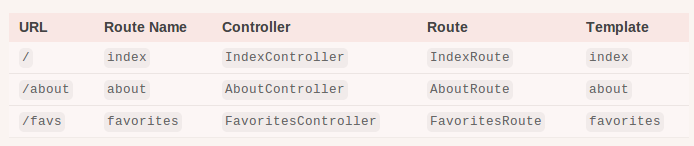
\includegraphics[width=1.0\textwidth]{./img/ember_routes_conventions.png}
	\caption{Ember Conventions for Routes, Source Ember Guides defining your routes}
	\label{fig:ember_routes}
\end{figure}


Starting the above mentioned code snippets would result in page showing empty input fields for the both properties, because we didn't define our model for the application. 
Every template is backed by a model, and the Route defines what model should be used by the template. As depicted in the table above, ember will look for an App.IndexRoute by convention, so this is the right place where we need to point to the model.

\begin{lstlisting}[label=em_controller,caption=app.js]
var App = Ember.Application.create();
App.Person = Ember.Object.extend({
	firstName: null,
	lastName : null,
    fullName: function() {
        return this.get('firstName') + " " + this.get('lastName');
    }.property('firstName','lastName')
});

var myself = App.Person.create({
    firstName: "Daniel",
    lastName: "Meiers",
});

App.IndexController = Ember.ObjectController.extend({});

App.IndexRoute = Ember.Route.extend({
    model: function() {
        return myself;
    }
});
\end{lstlisting}

Listing \ref{em_controller} needs some more explanation. First at all we define a Model class called Person which has the same properties as in the Knockout example. In order to do this, we need to extend a special ember class in fact we want to bind to these properties. After that, we create an instance of this class and set the needed Properties. In line 15 we declare the controller which should be used for the IndexRoute. In Ember a Controller is the component that stores the application state. It is comparable to Knockouts ViewModel object. As mentioned earlier, each template is backed by a model, which is not totally correct. To be exact, Templates retrieve their properties from the controller which decorated the model and provide proxy attributes to avoid writing "model.<property>" in the templates. In the IndexRoute object, we finally point the model property to our model instance.

\begin{figure}
	\centering	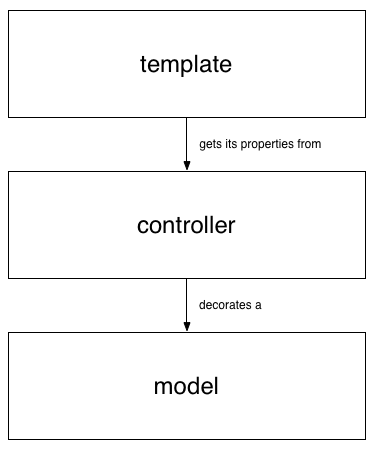
\includegraphics[width=0.4\textwidth]{./img/ember_controller_coupling.png}
	\caption{Ember model coupling, Source Ember Guides controllers}
	\label{fig:ember_coupling}
\end{figure} 
 

Per default it is not necessary to define the Controller for the IndexRoute, but by convention Ember assumes that the IndexController should manage a list of model objects and therfore expects an array for the model property. Another way to achieve the same thing, is demonstrated in the following listing. We simply define an special Ember Array and add our created Person instance to it, and finally point the IndexRoute to the array instead. Since we now have an array as our model, we need to adjust the template, to iterate over all existing array members (see listing \ref{em_array_template}).

\begin{lstlisting}[caption=app.js]
var persons = Ember.A();
persons.pushObject(myself);

App.IndexRoute = Ember.Route.extend({
    model: function() {
        return myself;
    }
});

\end{lstlisting}     

\begin{lstlisting}[label=em_array_template,caption=index.html]
<script type="text/x-handlebars" data-template-name="index">
	{{#each}}
		<div>
			<label>First Name</label> 
			<input {{bindAttr value=firstName}}></input>
		</div>
		<div>
			<label>Last Name</label> 
			<input {{bindAttr value=LastName}}></input>
		</div>
		<p>{{fullName}}</p>
	{{/each}}
</script>
\end{lstlisting}

If we start that application we see that the TextFields are properly bound to the model properties. But if we change the first name or last name in the TextField these changes are not reflected to the p-element at the bottom of the page. This is because Ember doesn't knwo how to react on events that are fired on user reaction. If we want to react on user events we need to use an Ember View. "Views are responsible for responding to user events, like clicks, drags, and scrolls, as well as updating the contents of the DOM when the data underlying the view changes." [ember guides - the view layer]
Luckily, Ember has a small set of built in views which are Ember.Checkbox, Ember.TextField, Ember.Select and Ember.Textarea. If necessary, it is also possible to create custom views. Therefore the only thing we need to change is to replace the input element with an Ember.TextField view as demonstrated in listing \ref{em_view}

\begin{lstlisting}[label=em_view,caption=Ember Views]
	{{view Ember.TextField valueBinding="firstName"}}
\end{lstlisting}

As mentioned earlier, Ember also provides a way to automatically connect Ember Models to an REST API, but in fact this module relies heavily on naming conventions and it is a not stable solution, I pass on showing some demo code.


\textbf{Angular JS}  

AngularJS is developed by Google and has become one of the more popular Frameworks (see github stars, forks). Angular JS follows a slightly different apporach compared to the other frameworks. This approach is best described by the Angular developers itself: "Angular is what HTML would have been had it been designed for applications" (angular documentation). One aspect that shows the difference of Qngular are the so called directives. Directives allow the user to extend the native HTML with new and application dependent functionality.  This is done by introducing new HTML tags or attributes, as well as some JavaScript code that defines the semantics/behaviour and a way how to convert the new introduced tag and the current model state into plain old HTML.  %(example?!). 
Using directives extensively, "HTML can be turned into a declarative domain specific language (DSL)" (Zitat angular doc)
  
The second aspect Angular differs from the other frameworks is the templating system. (angular docu says that the template system is DOM based ?)   

Besides these features Angular JS also provides two way data binding, filters, routing and dependency injection. 
All these components and features make it easy to write Single Page Web Applications without writing any sort of boilerplate code, assumed that you are familiar with the architecture and concepts of Angular JS. 
%(this is one the disadvantages, takes much time to get familiar with angular)  

%- is the one with the most community activity (github forks, stars, watches) 

Listing \ref{angularBasic} shows the very simple implementation of the same app used before. The special here is that we didn' need to write one line of JavaScript code to get things work. Unfortunately this example isn't very intuitive and it seems that there happens a lot of magic. In the following section I will explain the details of the example and the important concepts of Angular.

\begin{lstlisting}[label=angularBasic]
<html ng-app>
    <head>
        <meta charset="utf-8">
        <title>My AngularJS App</title>
    </head>
    <body ng-init="firstName='Daniel'; lastName='Meiers';">
        <div>
            <label>First Name</label> 
            <input ng-model="firstName"></input>
        </div>
        <div>
            <label>Last Name</label> 
            <input ng-Model="lastName"></input>
        </div>
        <p>Hello {{firstName}} {{lastName}}</p>
        <script src="lib/angular/angular.js"></script>
        <script src="js/app.js"></script>
    </body>
</html>
\end{lstlisting}

The first thing to mention here is the ng-app directive. This directive defines the application root and Angular automatically looks for this directive during page load. If found, it starts bootstrapping the angular application which basically means three things:
\begin{itemize}
	\item load the module associated with the directive.
	\item create the application injector
	\item compile the DOM treating the ng-app directive as the root of the compilation. 
\end{itemize}

Using this special directive as the root of the Angular related content has the advantage that only a part of the total Application can be handled by Angular. This makes it much easier to migrate Angular into existing projects or to combine Angular with other frameworks.

In Angular the application consists of one or more so called Modules. Modules "declaratively specify how an application should be bootstrapped" [source angular guides Modules]. This is necessary since Angular applications doesnt have a main method which can make the instantiation process. The Module that should be loaded can be referenced in the ng-app directive. 
\begin{lstlisting}[label=ngModule]
<html ng-app="myApp">
....
<script type="text">
	var myAppModule = angular.module('myApp', []);
</script>
....
\end{lstlisting}

The first parameter of the module creation (line 4 of listing \ref{ngModule}) defines the name of the module we have to use for referencing it in the ng-app directive. The second parameter can be used to define other modules as dependency for this module. These dependent modules are created first and then injected into the module per Dependency Injection.


The most notably advantage among others of this procedure is, that the seperation in modules simplifies unit testing, since not all modules must be loaded for unit testing and additional modules can be loaded ,that can override some of the configuration. This helps writing end-to-end test the application (testing the gui behaviour.) 


In our simple application (see listing \ref{angularBasic}) we haven't defined what module should be loaded, therefore angular loads a default module. An "ng-app Module" is used to initialize the application wide Injector which is responsible for the Dependency Injection. The last step of bootstrapping comprises the (re-)compilation of the DOM. Each found Directive or binding expression is evaluated and translated into plain HTML.


The next directive we used in \ref{angularBasic} is the ng-init directive. It allows to do initilisation tasks before the app starts running. In this case it automically creates a new ViewModel called Scope, add its the two properties and most important, sets the respective inital values for it. The ng-model directive binds a property of the Scope to this element, which automatically enables a two-way data binding between them. If the property of the ng-model directive doesn't exist, it creates it automatically. This feature is a great difference compared to Knockout and Ember. Before explaining this feature in more deatail it is necessary to define what a Scope in Angular means. Therefore it is also necessary to understand what Models, Controller and Views are in Angulars architecutre.


The Scope is an object that refers to the application model and provides necessary context for data binding expressions and directives. They can watch Angular Expressions and propagate events. These features are used to implement the two way databinding. Scopes are the "glue between application controller and the view"[source angular doku] and are comparable to Knockouts ViewModel. An Angular application contains of exactly one RootScope and a set of (multiple)  ChildScopes. They are hirarchical nested and resemble the DOM structure (see Figure \ref{fig:angular_scopes}). Similar to the model declaration, this can also happen implicit by directives like the ng-repeat directive in figure \ref{fig:angular_scopes}. ChildScopes prototypically inherit from their parent scope. Hence, if an binding expression like {{firstName}} is evaluated by Angular it first checks if the Scope object related to that element contains this property. If not it checks all ParentScopes until the property is found or the RootScope is reached.

\begin{figure}
	\centering	
	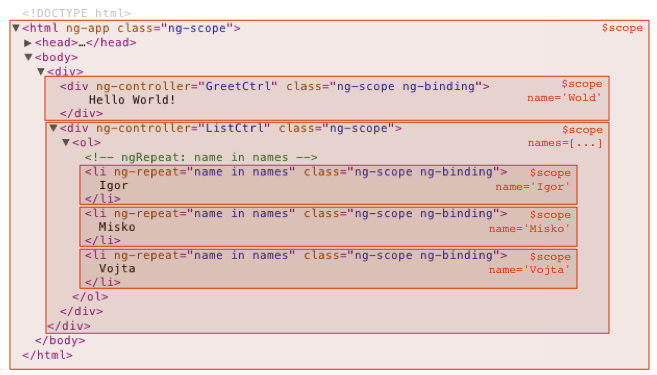
\includegraphics[width=0.8\textwidth]{./img/angular_scopes.png}
	\caption{Hirarchie of Angular scopes}
	\label{fig:angular_scopes}
\end{figure} 

In Angular a Model can be any JavaScript object inlcuding Arrays and primitives. The only condition is that it must be referenced by a Scope object. The name of the scope property is the model identifier. The creation of models can be done explicit or implicit. In our example we created the model implicit with the ng-model directive. To create a Model explicit you usually add new Properties to the Scope in it's Controller. A good overview over the different possibilites to create models can be found at [see angular guides understanding model component]


As already mentioned, Controllers are also a way to create models in Angular and adding them to the Scope. Controllers are simple JavaScript functions that are used to augment the angular scope and are normally used to set up inital state of the Scope or to add application behaviour to it. Listing \ref{angularController} depicts the needed changes.

\begin{lstlisting}[label=angularController,caption=Angular Controller]
<html>
....
<body ng-controller="HelloController">
....
<script type="text">
	function HelloController($scope){
	    $scope.lastName = "Meiers";
	    $scope.firstName = "Daniel";
	};
</script>
...
\end{lstlisting}

There are two ways how Controllers are associated with Scope objects. The first one is to use the ng-controller directive as in the example above. The second one is to use Angulars Routing mechanism. Another important thing to mention here is that the Scope object is provided by Angulars DI (Dependenci Injection) system.   

The last component to cover all elements of the MVC pattern is the View. In Angular the view consists of the loaded and rendered DOM after Angular has transformed Angular specific directives and expression using Scopes,Controllers, and Models. Fig. \ref{fig:angular_views} and Fig\ref{fig:angular_views_2} gives a good overview over this process.
  
\begin{figure}
	\centering	
	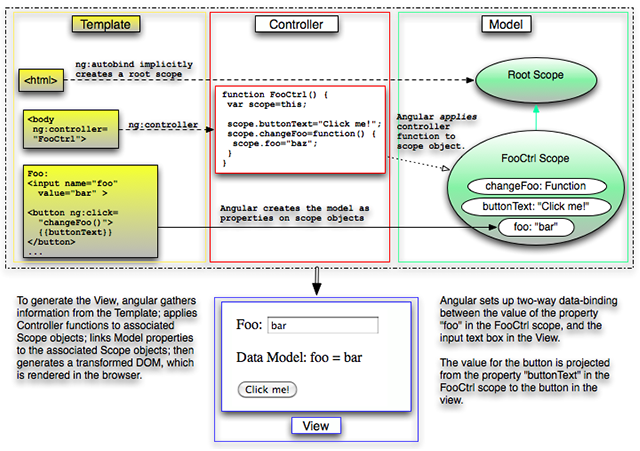
\includegraphics[width=0.8\textwidth]{./img/angular_view.png}
	\caption{Functionality of Angular Views}
	\label{fig:angular_views}
\end{figure} 

\begin{figure}
	\centering	
	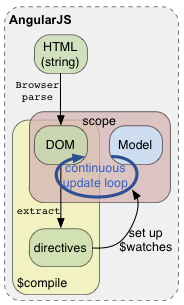
\includegraphics[width=0.3\textwidth]{./img/angular_view_2.png}
	\caption{Functionality of Angular Views}
	\label{fig:angular_views_2}
\end{figure} 

There are a few more concepts in Angular that helps and simplifies SPA development with Angular. A really usefull feature that makes Angular outstanding are Filters.
Filters are a way to format data that should be displayed to the user. For example, if we want to print the fullName property of our basic example in uppercase letters we just need to use the Uppercase filter provided by Angular (see listing \ref{angular_filters}). Angular already provides a basic set of very useful Filters among them Filters for ordering or filtering lists of data but it is also possible to create custom ones. Filters are used in Angular templates with an Bash like pipe syntax.

\begin{lstlisting}[label=angular_filters,caption=Angular Filters]
 {{ fullName | uppercase}}
\end{lstlisting}

The last concept are Services. Services in Angular apps are substitutable objects that are wired together using dependency injection (DI).Angular services are singletons that carry out specific tasks common to web apps, such as the \$http service that provides low level access to the browser's XMLHttpRequest object. This service can be used to load json objects.

%-> Angular Routing



The following table gives an overview over the different features of each framework compares them.

\begin{landscape}
	\begin{longtable}{| p{5cm} | p{5cm} | p{5cm} | p{5cm} |}
	\hline
		& Angular JS				
		& Ember JS	
		& Knockout JS \\ \hline
	2-way binding	 		
		& \checkmark
		& \checkmark
		& \checkmark  \\ \hline
	normal / computed properties	
		& \checkmark / change detection
		& \checkmark / \checkmark
		& \checkmark / \checkmark\\ \hline
	Testing				
		& very easy, end-to-end test, build in tools for unit tests, 
		  end to end test (gui tests), tools for testing app in realtime with different browsers 
		& extra packages ember-testing,qUnit 
		&  unit tests \\ \hline
	Routing				
		& \checkmark 
		& \checkmark	
		& -		\\ \hline
	Multiple / Composite Views	
		& \checkmark / \checkmark
		& \checkmark / \checkmark 
		& -		\\ \hline
	Backend connection		
		& optional (ajax wrapper)	
		& optional (ember-data)	
		& -	\\ \hline
	Dependency injection
		& \checkmark
		& -
		& -\\ \hline
	Templating system
		& Dom based 
		& String based (handlebars)
		& Dom based\\ \hline
	Documentation
		& very good
		& good
		& good\\ \hline
	API stability / maturity
		& Initial release 2009, curr 1.0.7
		& Inital release 2011, curr ember 1.0.0-rc6.1
		& First version 2010, current 2.3.0\\ \hline
	community (github watch/star/fork
		& 1450/13061/3147
		& 672/7752/1568
		& 349/4074/657\\ \hline
	Security
		&
		&
		& \\ \hline
	Perfomance
		&
		&
		& \\ \hline
	Flexibile vs opinonated
		& flexible
		& stringent \& opinionated
		& very flexible\\ \hline
	size
		& 80kb
		& 56kb + JQuery + Handlebars
		& 15kb\\ \hline	
	FrameWork / Library
		& Something in between
		& Framework
		& Library\\ \hline
	Allows integration of ui elements
		& \checkmark use directives
		& \checkmark use Ember views
		& \checkmark use custom bindings \\ \hline
	\end{longtable}
\end{landscape}



\section{Discussion}

Knockout JS very reduced feature set can be both, a blessing and a curse and it depends on the needs to decide what of these two things prevails. Knockout JS is a very easy to learn library hence there are only a few concepts to learn. Another benefit of Knockout JS is, that it has a widely spreaded browser support also for older browser versions. This benefit is not that much relevant since the apps to develop should be rendered in the JavaFX WebKit component. Knockout is a very flexible framework hence there are  no regulations for defining the structure and architecture of your application. The missing features of Knockout JS like routing can be compensated with one of the other dozen available third party libraries for this feature. Unfortunately, without these additional dependencies Knockout JS is rather less suited for building web applications in fact that it forces you to implement too many things manually. And the additional amount of dependencies could lead to inconsitency problems, increases the error likelyhood and the maintenance efforts and make the development event harder. (vgl artice heise online)     


Ember however, covers all needed aspects of developing SPA's. It is possible to write applications with a minimal amount of code, and its concept scale very well, which means it is very easy to write simple Applications with Ember, but the underlaying concepts cover also the possibilty to create large and complex Single Page Web Applications. The problem is, that Ember is a very strict and opinonated Framework, this is especially true for ember-data which relies heavily on naming conventions to work. Using approaches like Convention over Configuration is not a disadvantage but the question is, if the very stringent corsett of ember will limit further developments or produces a lot of efforts to work around these framework limitations. A good example for this is ember-data. Since ember-data is not a stable solution it would be necessary to implement an own backend connection anyway if choosing Ember. But if we exclude that fact using ember-data would dictate the structure of the backends REST API. And the propblem is, if this structure needs to be changed for any other reason, it is necessary work around this issue. Even if it is not very likely, but the same could happen for example with Embers Routing mechanism. 


At this point, the concept of Dependency Injection, and Services, makes Angular much more flexible. Similar to Ember, with Angular you are also capable of building all kind of applications, from the simple to the complex one. It's alternative way of directives seems very attractive. All these concepts makes it a bit harder to get familiar with Angular, but if the concepts are clear, it is very intuitive to build applications with Angular. Outstanding points of Angular are besides directives, the usage of Dependency Injection, which allows to easily reuse developed Filters, Services and so on. Furthermore DI increases the testability a lot. 


Testing an Angular Application with the choosen JavaFX WebKit component has shown, that it is not possible to debug them with the very well known Firebug tool (No debugging tools in JavaFx WebKit like in other Browsers, Firebug the most promising JavaScript debugging tool). Further research about this issue has shown, that Angular and Firebug seems to be incompatible, in fact Angular add some specific styling elements to the DOM, that Firebug can't parse. This a really large problem which need to be solved if choosing Angular.   


%\chapter{Implementation}

%\chapter{Discussion}


%\listoffigures
\printbibliography

\end{document}
